\chapter{Testing and Evaluation}\label{testing}

    \section{Performace Evaluation}
        - Sequential vs Parallel
            -	31 frames process vs 16 frames process
            -	Caffe MobileNet SSD vs Darknet YOLO model
                - YOLO
                    - use more memory because it calls lots of native libs (C++) which is very expensive.
                        - GC collect very often
                        - Programme is frozen
                    - More accuracy
                        - Able to detect person with confidence threshold 0.5
                - SSD
                    - Use less memory
                        - No GC collecting
                    - Less accuracy
                        - Able to detect person with confidence threshold 0.3


        % Picture Performance Table
        \begin{table}[!htp]\centering
            \scriptsize
            \begin{tabular}{lrrrrrr}\toprule
                \multicolumn{2}{c}{Model} &\multicolumn{2}{c}{YOLO} &\multicolumn{2}{c}{SSD} \\\midrule
                \multicolumn{2}{c}{Size} &960×540 &540x480 &960×540 &540x480 \\
                \multicolumn{2}{c}{Total Process Time (second)} &4.235 &3.827 &0.337 &0.323 \\
                \multicolumn{2}{c}{Forward Propagation per frame (second)} &3.456 &3.019 &0.284 &0.278 \\
                \multicolumn{2}{c}{Forward Propagation per frame (perenctage)} &81.61\% &78.89\% &84.27\% &86.07\% \\
                \bottomrule
            \end{tabular}

            \caption{Picture Processing Performace}\label{performance:picture}
        \end{table}

        % YOLO Model Performace Table
        \begin{table}[!htp]\centering
            \scriptsize
            \begin{tabular}{lrrrrrrrr}\toprule
                \multicolumn{2}{c}{Model} &\multicolumn{6}{c}{YOLO} \\\cmidrule{1-8}
                \multicolumn{2}{c}{\multirow{2}{*}{}} &\multirow{2}{*}{Sequential Computing} &\multicolumn{5}{c}{Parallel Computing} \\\cmidrule{4-8}
                & & &1 Thread &2 Threads &4 Threads &6 Threads &8 Threads \\\midrule
                \multicolumn{2}{c}{Total Process Time (second)} &102.972 &117.805 &96.415 &92.242 &88.688 &99.441 \\
                \multicolumn{2}{c}{Garbage Collector (second)} &- &0.102 &0.280 &2.024 &3.625 &11.333 \\
                \multicolumn{2}{c}{Process Time without GC} &- &117.703 &96.136 &90.218 &85.065 &88.108 \\
                \multicolumn{2}{c}{Forward Propagation (Total)} &79.097 &- &- &- &- &- \\
                \multicolumn{2}{c}{Forward Propagation (Average)} &2.553 &2.872 &4.840 &9.231 &12.827 &19.713 \\
                \multicolumn{2}{c}{Forward Propagation (Min)} &2.213 &2.564 &4.003 &5.478 &8.301 &14.733 \\
                \multicolumn{2}{c}{Forward Propagation (Max)} &2.693 &3.092 &6.436 &12.566 &15.324 &21.815 \\
                \multicolumn{2}{c}{Number of frame} &31 &31 &31 &31 &31 &31 \\
                \multicolumn{2}{c}{Process per frame (second)} &3.322 &3.800 &3.110 &2.976 &2.861 &3.208 \\
                \bottomrule
            \end{tabular}

            \caption{Video Processing with YOLO Model}\label{yolo:performance}
        \end{table}

        % SSD Model Performace Table
        \begin{table}[!htp]\centering
            \scriptsize
            \begin{tabular}{lrrrrrrrr}\toprule
                \multicolumn{2}{c}{Model} &\multicolumn{6}{c}{MobileNet SSD} \\\cmidrule{1-8}
                \multicolumn{2}{c}{\multirow{2}{*}{}} &\multirow{2}{*}{Sequential Computing} &\multicolumn{5}{c}{Parallel Computing} \\\cmidrule{4-8}
                & & &1 Thread &2 Threads &4 Threads &6 Threads &8 Threads \\\midrule
                \multicolumn{2}{c}{Total Process Time (second)} &7.132 &8.237 &6.873 &6.270 &5.137 &5.064 \\
                \multicolumn{2}{c}{Garbage Collector (second)} &- &- &- &- &- &- \\
                \multicolumn{2}{c}{Process Time without GC} &- &- &- &- &- &- \\
                \multicolumn{2}{c}{Forward Propagation (Total)} &7.019 &- &- &- &- &- \\
                \multicolumn{2}{c}{Forward Propagation (Average)} &0.226 &0.235 &0.401 &0.738 &0.900 &1.133 \\
                \multicolumn{2}{c}{Forward Propagation (Min)} &0.218 &0.212 &0.353 &0.406 &0.428 &0.466 \\
                \multicolumn{2}{c}{Forward Propagation (Max)} &0.243 &0.320 &0.456 &1.477 &3.057 &2.582 \\
                \multicolumn{2}{c}{Number of frame} &31 &31 &31 &31 &31 &31 \\
                \multicolumn{2}{c}{Process per frame (second)} &0.230 &0.266 &0.222 &0.202 &0.166 &0.163 \\
                \bottomrule
            \end{tabular}

            \caption{Video Processing with MobileNet SSD Model}\label{ssd:performance}
        \end{table}

        -	Limitation / Problem
            - Limited Resource
                - CPU clock speed
                - RAM
                - Power resources

            - CPU
                - ARM architecture limitation on floating-point [http://tinyurl.com/y85ykaqa]
                - When the number of threads is increasing, image processing task is not consistently processed by core.
                    - Because the given task has to wait while core switching and doing another task (context switching)
                    - Thus, the given task requires more time to be finished
            - JNI
                - Calling JNI is expensive [ref]

            -	Multithread Performance Analysis
                - I/O in thread
                    - If there is I/O operation in thread or loop, it will cost a lot of overhead
                - Out of memory
                    - If let each thread hold the large variable, it will cost memory overhead.
                    - We have to free the variables after used. Otherwise, the x+1 th thread will allocate another xx MB.
                - Young generation
                    - If there are lot of variables that are initialled in loop, there will be a lot young generation in the heap. So, when the number of young generations is reaching the threshold, GC will correct the young generation (freeing garbage in young generation heap) which affect the performance.
                - GC
                    - Caused by Native [https://developer.android.com/studio/profile/memory-profiler]
                    - Bin is GC
                    - 8 GB (available only 3.8 GB)
                - CPU hits 100% when performing tasks
                - CPU drops when GC is started
                        - Because threads are paused (Yellow) when GC is collecting

        % Memory Usgae
        \begin{figure}[!ht]
            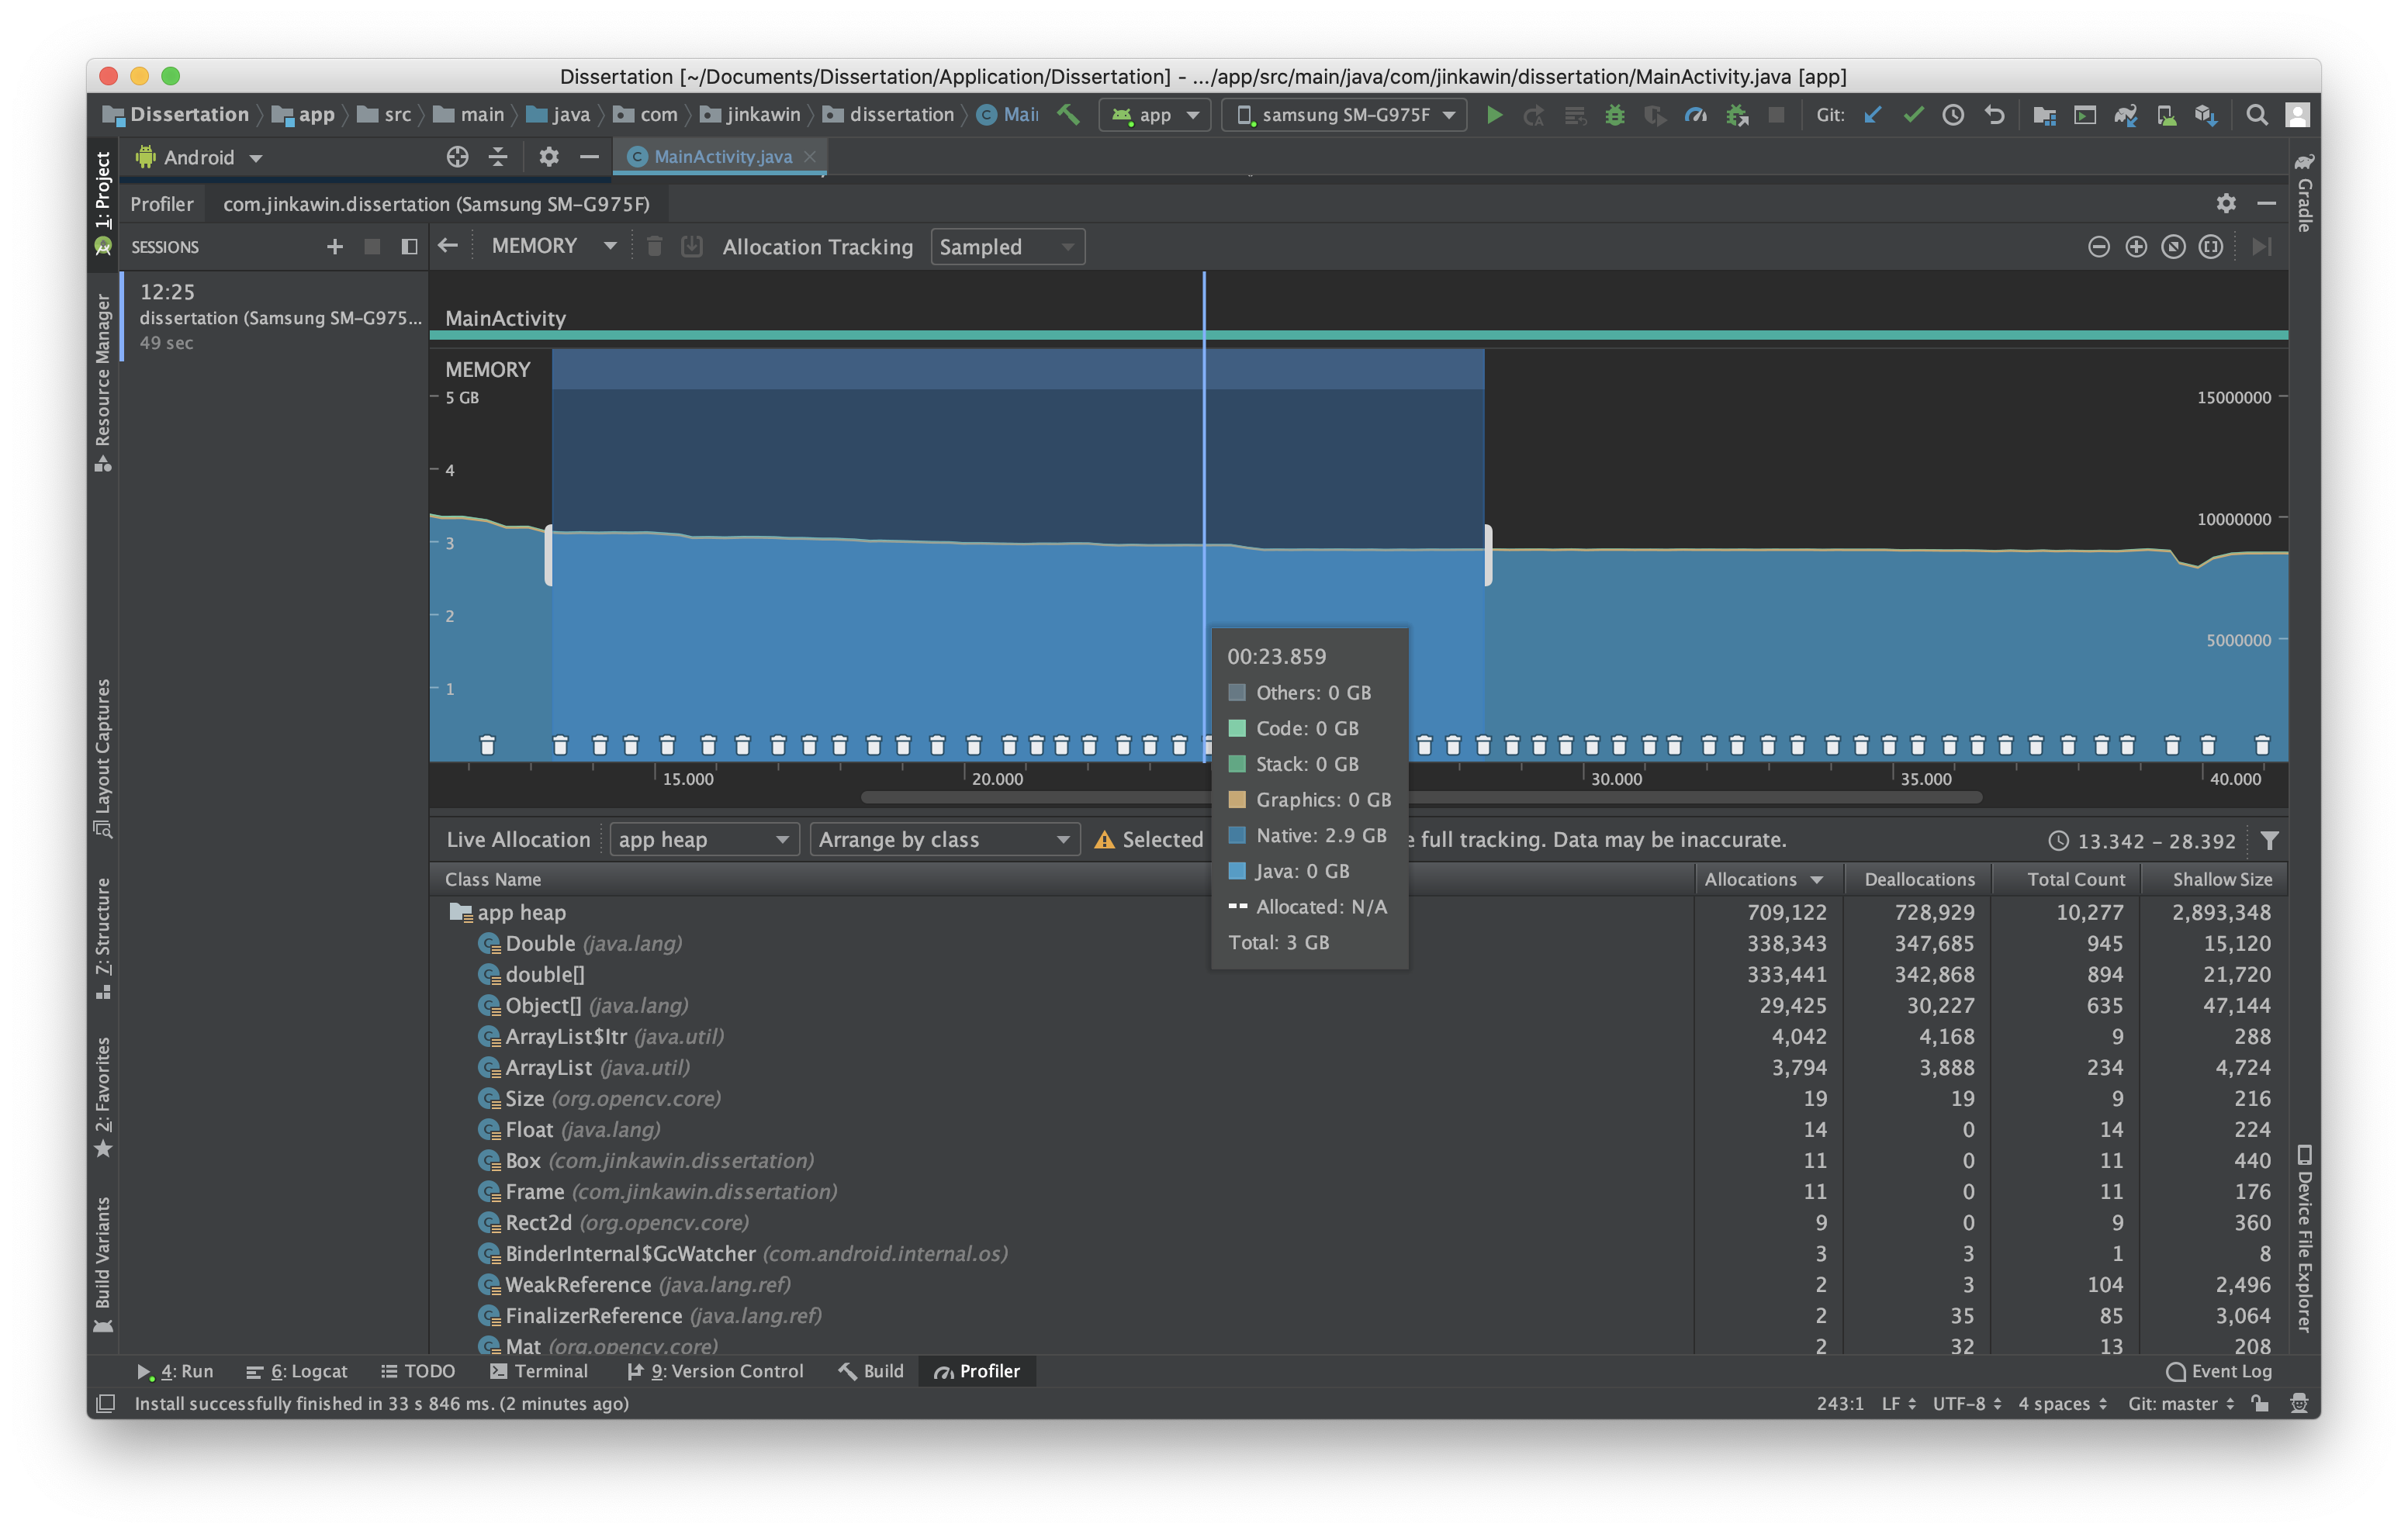
\includegraphics[width=6in]{images/chapter5/gc-problem/gc-collecting.png}
            \caption{YOLO Model's Memory Usage}
            \label{yolo:memoryUsage}
        \end{figure}

        % CPU Usage
        \begin{figure}[!ht]
            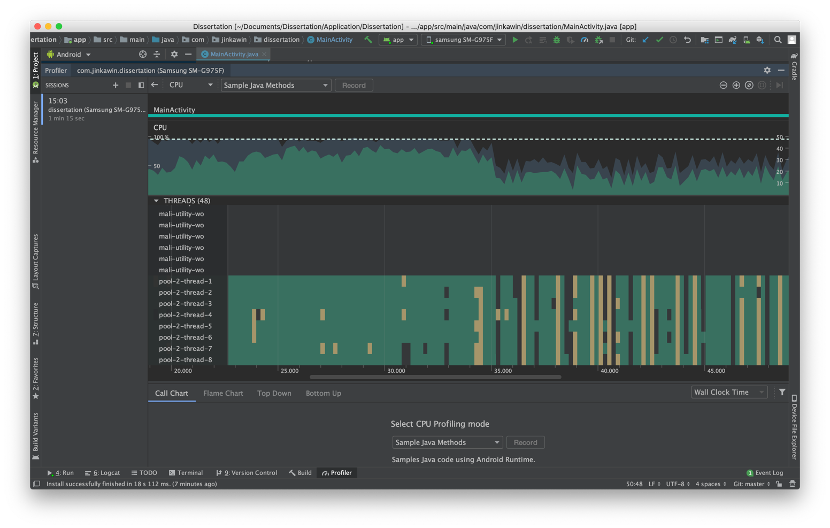
\includegraphics[width=6in]{images/chapter5/YOLO/cpu-usage-8threads.png}
            \caption{YOLO Model's CPU Usage}
            \label{yolo:cpuUsage}
        \end{figure}

    \section{Usability Testing}